\section{Redes sociais (GODSocialNetIO)}
\label{sec-1}
\subsection{Team}
\label{sec-1-1}

  Eduardo Alexandre, Aline Borges, Leonardo Haddad, Thiago Araujo
\subsection{Description}
\label{sec-1-2}

  Our module for the GOD Project is to allow others modules to communicate with the Facebook and Twitter servers. It does that by implementing both public APIs.\\

  The module is divided in two main parts, first are the fetchers, these classes are responsable to all the communication with the APIs.\\

  Then there are the GODData clases, these ones receive the JSON response from a request made by a fetcher and transforms it into a GODData type of object.\\

  It's important to mention that both Facebook and Twitter APIs need a client id and secret to work, this can be done creating a specific type of user in the developer section of both APIs.\\

  Last but not least, we have classes responsable to test all the methods within the fetchers and GODDatas, keep in mind that we don't have control of the Facebook and Twitter servers, so some test may fail some times simply because the server response is not what was spected.
\subsection{Class Diagram}
\label{sec-1-3}

\begin{center}
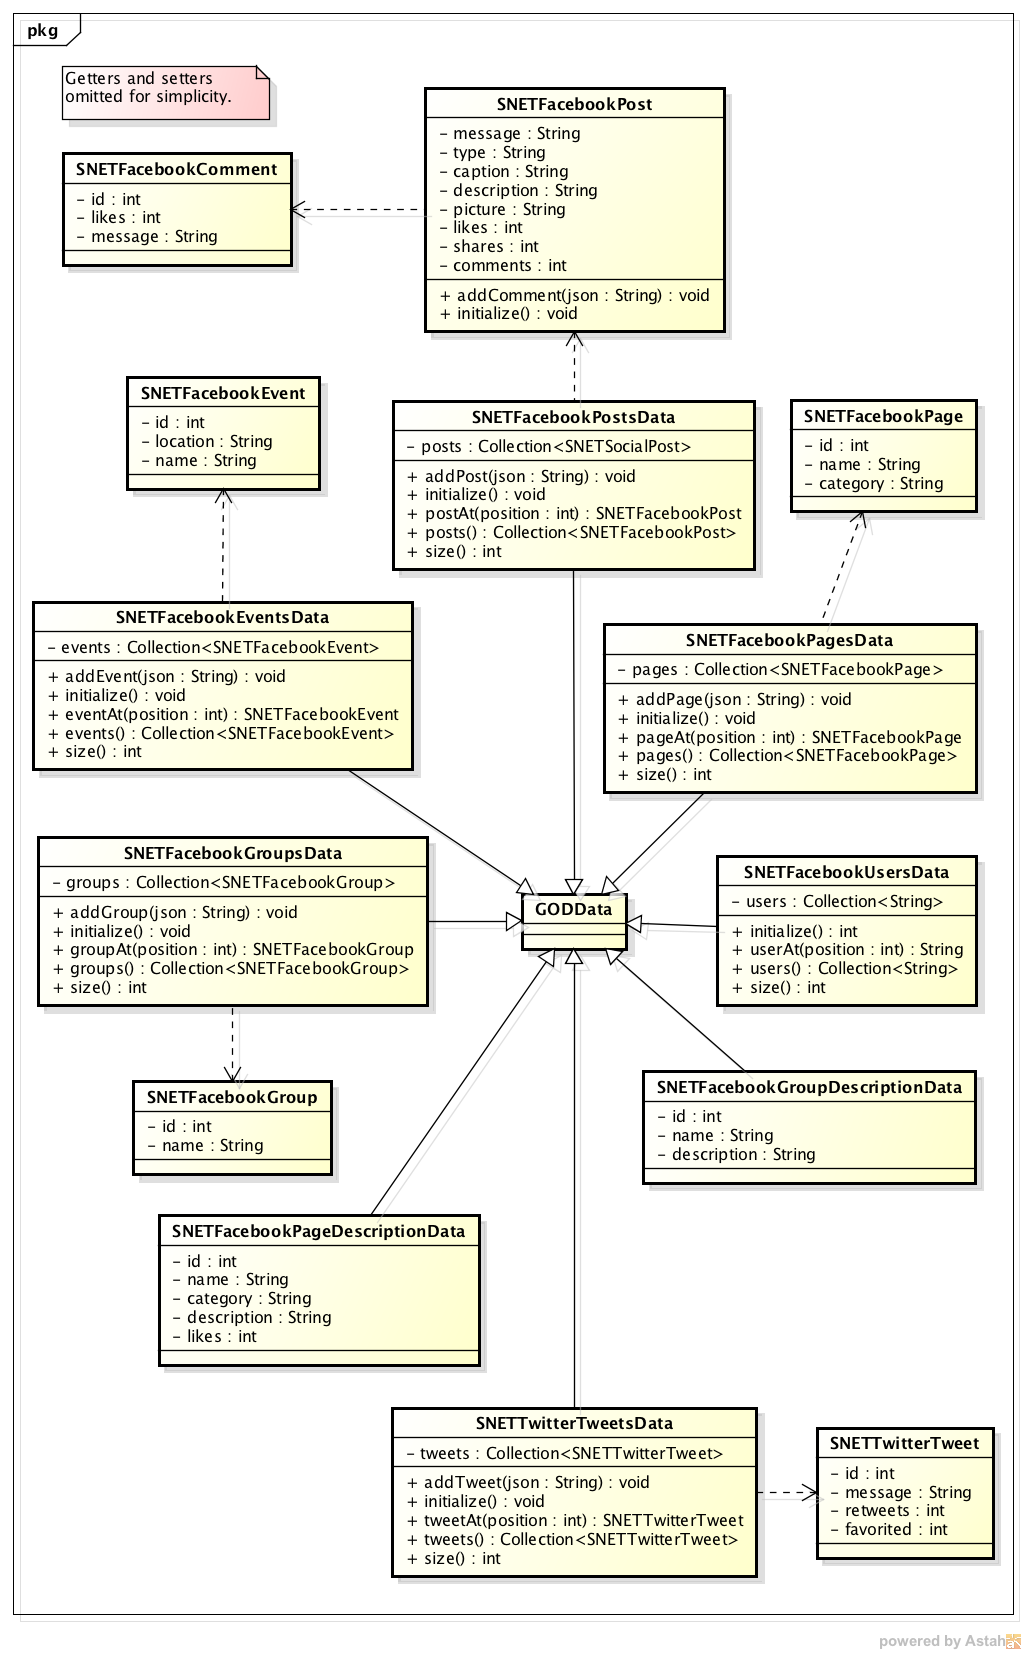
\includegraphics[width=.9\textwidth]{SocialNetIO-1.png}
\end{center}

\begin{center}
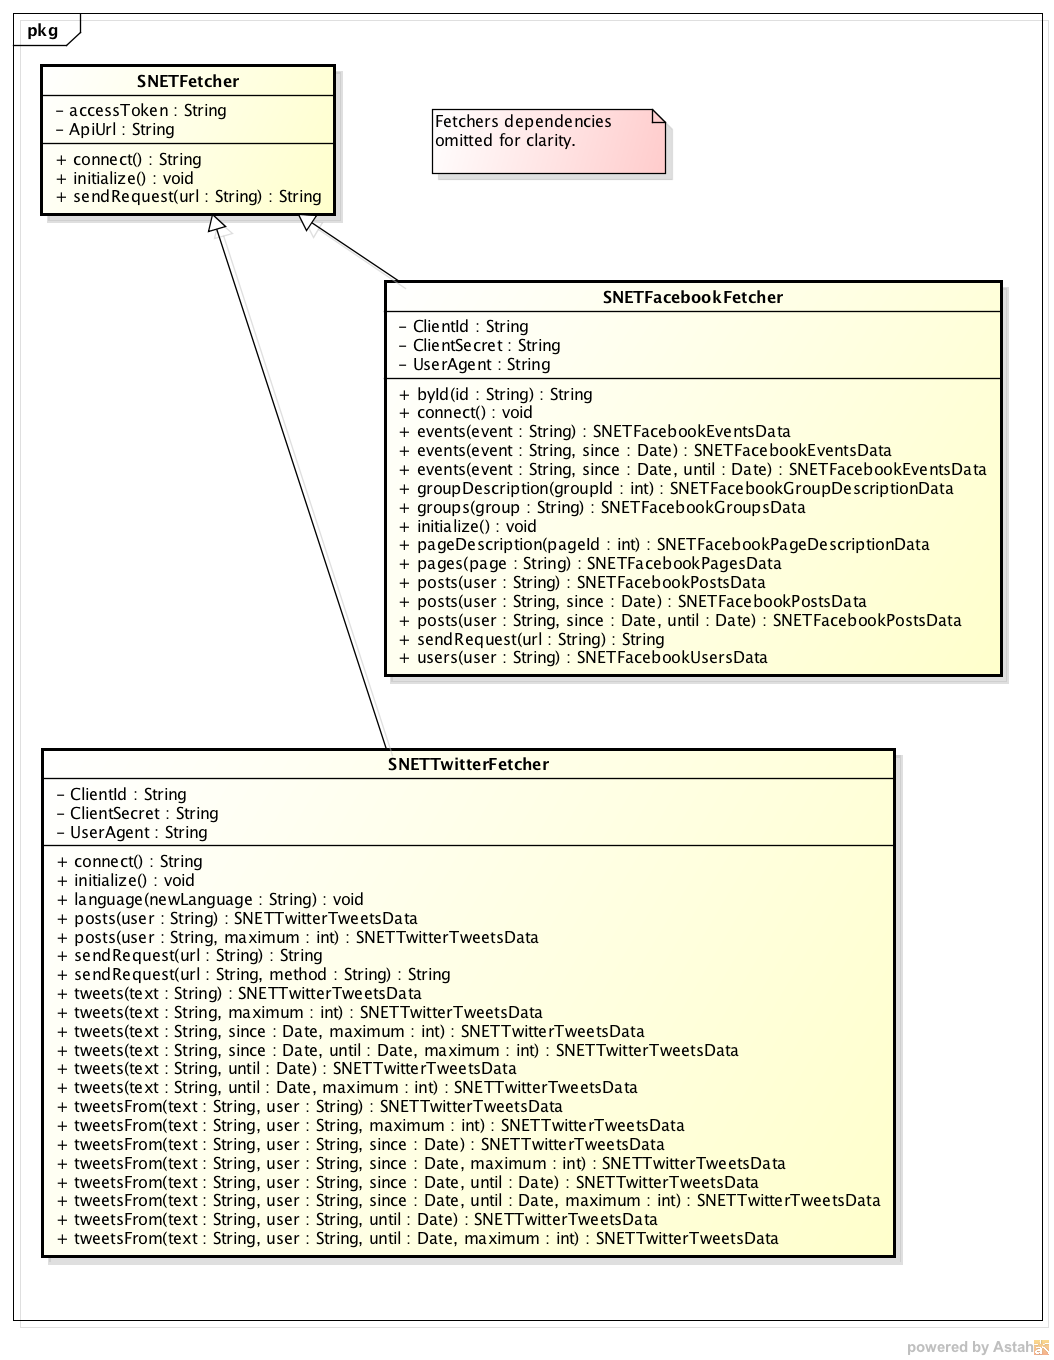
\includegraphics[width=.9\textwidth]{SocialNetIO-2.png}
\end{center}
\subsection{Documentation}
\label{sec-1-4}
\subsubsection{Fetchers}
\label{sec-1-4-1}
\begin{itemize}

\item Class SNETFetcher\\
\label{sec-1-4-1-1}%
SNETFetcher is a abstract class that contains the common parts used by SNETFacebookFetcher and SNETTwitterFetcher.

\begin{itemize}

\item Instance Variables
\label{sec-1-4-1-1-1}%
\begin{itemize}
\item \verb~accessToken~\\\\
\textbf{Type:}\\
     String.\\

     \textbf{Description:}\\
     This variable will store the access token necessary to access Facebook or Twitter servers.
\end{itemize}


\item Class Variables
\label{sec-1-4-1-1-2}%
\begin{itemize}
\item \verb~ApiUrl~\\\\
\textbf{Type:}\\
     String.\\

     \textbf{Description:}\\
     This variable will store the full URL to either Facebook or Twitter servers.
\end{itemize}


\item Functions
\label{sec-1-4-1-1-3}%
\begin{itemize}

\item private
\label{sec-1-4-1-1-3-1}%
\begin{itemize}
\item \verb~sendRequest: url~\\\\
\textbf{Description:}\\
      This abstract function job is to send some HTTP request to some url, it will be specialized in SNETFacebookFetcher and SNETTwitterFetcher.
\end{itemize}


\item initialize-release
\label{sec-1-4-1-1-3-2}%
\begin{itemize}
\item \verb~initialize~\\\\
\textbf{Description:}\\
      This is the default function to initialize the class.
\end{itemize}


\item connection
\label{sec-1-4-1-1-3-3}%
\begin{itemize}
\item \verb~connection~\\\\
\textbf{Description:}\\
      This abstract function job is to connect to some server.
\end{itemize}


\end{itemize} % ends low level
\end{itemize} % ends low level

\item Class SNETFacebookFetcher\\
\label{sec-1-4-1-2}%
SNETFacebookFetcher is a class that controls all the access to the Facebook API.\\
   
   It sends requests to the facebook server and returns the result as a SNETFacebookUsersData object, SNETFacebookPostsData, SNETFacebookPagesData, SNETFacebookPageDescriptionData, SNETFacebookGroupsData, SNETFacebookGroupDescriptionData and SNETFacebookEventsData.

\begin{itemize}

\item Class Variables
\label{sec-1-4-1-2-1}%
\begin{itemize}
\item \verb~ClientId~\\\\
\textbf{Type:}\\
     String.\\

     \textbf{Description:}\\
     This variable will store the client id needed to connect to the Facebook API.\\
\item \verb~ClientSecret~\\\\
\textbf{Type:}\\
     String.\\

     \textbf{Description:}\\
     This variable will store the client secret needed to connect to the Facebook API.\\
\item \verb~UserAgent~\\\\
\textbf{Type:}\\
     String.\\

     \textbf{Description:}\\
     This variable will store the user agent used by \verb~sendRequest~ function to send HTTP requests to the Facebook API.
\end{itemize}


\item Functions
\label{sec-1-4-1-2-2}%
\begin{itemize}

\item private
\label{sec-1-4-1-2-2-1}%
\begin{itemize}
\item \verb~sendRequest: url~\\\\
\textbf{Description:}\\
      This function job is to send some HTTP request to Facebook API.\\
\item \verb~byId: id~\\\\
\textbf{Description:}\\
      This function job is to be a helper to some functions that search in the Facebook API using some id.
\end{itemize}


\item initialize-release
\label{sec-1-4-1-2-2-2}%
\begin{itemize}
\item \verb~initialize~\\\\
\textbf{Description:}\\
      This is the default function to initialize the class, it will initialize all the class variables.
\end{itemize}


\item connection
\label{sec-1-4-1-2-2-3}%
\begin{itemize}
\item \verb~connection~\\\\
\textbf{Description:}\\
      This function job is to connect to Facebook API.\\
\end{itemize}


\item accessing
\label{sec-1-4-1-2-2-4}%
\begin{itemize}
\item \verb~events: event~\\\\
\textbf{Description:}\\
      This function job is to search for events with the parameter name.\\
\end{itemize}


\begin{itemize}
\item \verb~events: event since: since~\\\\
\textbf{Description:}\\
      This function job is to search for events with the parameter name since some date.\\
\item \verb~events: event since: since until: until~\\\\
\textbf{Description:}\\
      This function job is to search for events with the parameter name since some date until another date.\\
\item \verb~groupDescription: groupId~\\\\
\textbf{Description:}\\
      This function job is to get group information by id.\\
\item \verb~groups: group~\\\\
\textbf{Description:}\\
      This function job is to search for groups with the parameter name.\\
\item \verb~pageDescription: pageId~\\\\
\textbf{Description:}\\
      This function job is to get page information by id.\\
\item \verb~pages: page~\\\\
\textbf{Description:}\\
      This function job is to search for pages with the parameter name.\\
\item \verb~posts: user~\\\\
\textbf{Description:}\\
      This function job is to get posts from user.\\
\item \verb~posts: user since: since~\\\\
\textbf{Description:}\\
      This function job is to get posts from user since some date.\\
\item \verb~posts: user since: since until: until~\\\\
\textbf{Description:}\\
      This function job is to get posts from user since some date until another date.\\
\item \verb~users: user~\\\\
\textbf{Description:}\\
      This function job is to search for users with the parameter name.\\
\end{itemize}


\end{itemize} % ends low level
\end{itemize} % ends low level

\item Class SNETTwitterFetcher\\
\label{sec-1-4-1-3}%
SNETTwitterFetcher is a class that control all the access to the Twitter API.\\

   It send requests to the twitter server and return the result as data class SNETTwitterTweetsData.

\begin{itemize}

\item Instance Variables
\label{sec-1-4-1-3-1}%
\begin{itemize}
\item \verb~tokenType~\\\\
\textbf{Type:}\\
     String.\\

     \textbf{Description:}\\
     This variable will store the token type necessary to perform different requests from the Twitter server.\\
\item \verb~lang~\\\\
\textbf{Type:}\\
     String.\\

     \textbf{Description:}\\
     This variable will store the language used when searching for tweets.
\end{itemize}


\item Class Variables
\label{sec-1-4-1-3-2}%
\begin{itemize}
\item \verb~ClientId~\\\\
\textbf{Type:}\\
     String.\\

     \textbf{Description:}\\
     This variable will store the client id needed to connect to the Twitter API.
\item \verb~ClientSecret~\\\\
\textbf{Type:}\\
     String.\\

     \textbf{Description:}\\
     This variable will store the client secret needed to connect to the Twitter API.
\item \verb~UserAgent~\\\\
\textbf{Type:}\\
     String.\\

     \textbf{Description:}\\
     This variable will store the user agent used by \verb~sendRequest~ function to send HTTP requests to the Twitter API.
\end{itemize}


\item Functions
\label{sec-1-4-1-3-3}%
\begin{itemize}

\item private
\label{sec-1-4-1-3-3-1}%
\begin{itemize}
\item \verb~sendRequest: url~\\\\
\textbf{Description:}\\
      This function job is to send some HTTP request to Twitter API.\\
\item \verb~sendRequest: url method: method~\\\\
\textbf{Description:}\\
      This function job is to send some HTTP request with either GET or POST method to Twitter API.\\
\end{itemize}


\item initialize-release
\label{sec-1-4-1-3-3-2}%
\begin{itemize}
\item \verb~initialize~\\\\
\textbf{Description:}\\
      This is the default function to initialize the class, it will initialize all the class and instance variables.
\end{itemize}


\item connection
\label{sec-1-4-1-3-3-3}%
\begin{itemize}
\item \verb~connection~\\\\
\textbf{Description:}\\
      This function job is to connect to Twitter API.\\
\end{itemize}


\item accessing
\label{sec-1-4-1-3-3-4}%
\begin{itemize}
\item \verb~posts: user~\\\\
\textbf{Description:}\\
      This function job is to get posts from user.\\
\item \verb~posts: user maximum: max~\\\\
\textbf{Description:}\\
      This function job is to get posts from user specifying the maximum amount of posts.\\
\item \verb~tweets: text~\\\\
\textbf{Description:}\\
      This function job is to get tweets from text.\\
\item \verb~tweets: text maximum: max~\\\\
\textbf{Description:}\\
      This function job is to get tweets from text specifying the maximum amount of tweets.\\
\item \verb~tweets: text since: date maximum: max~\\\\
\textbf{Description:}\\
      This function job is to get tweets from text since date specifying the maximum amount of tweets.\\
\item \verb~tweets: text since: initDate until: endDate maximum: max~\\\\
\textbf{Description:}\\
      This function job is to get tweets from text since date until another date specifying the maximum amount of tweets.\\
\item \verb~tweets: text until: date~\\\\
\textbf{Description:}\\
      This function job is to get tweets from text until date.\\
\item \verb~tweets: text until: date maximum: max~\\\\
\textbf{Description:}\\
      This function job is to get tweets from text until date specifying the maximum amount of tweets.\\
\item \verb~tweetsFrom: text user: user~\\\\
\textbf{Description:}\\
      This function job is to get tweets from text from user.\\
\item \verb~tweetsFrom: text user: user maximum: max~\\\\
\textbf{Description:}\\
      This function job is to get tweets from text from user specifying the maximum amount of tweets.\\
\item \verb~tweetsFrom: text user: user since: date~\\\\
\textbf{Description:}\\
      This function job is to get tweets from text from user since date.\\
\item \verb~tweetsFrom: text user: user since: date maximum: max~\\\\
\textbf{Description:}\\
      This function job is to get tweets from text from user since date specifying the maximum amount of tweets.\\
\item \verb~tweetsFrom: text user: user since: initDate until: endDate maximum: max~\\\\
\textbf{Description:}\\
      This function job is to get tweets from text from user since date until another date specifying the maximum amount of tweets.\\
\item \verb~tweetsFrom: text user: user until: date~\\\\
\textbf{Description:}\\
      This function job is to get tweets from text from user until date.\\
\item \verb~tweetsFrom: text user: user until: date maximum: max~\\\\
\textbf{Description:}\\
      This function job is to get tweets from text from user until date specifying the maximum amount of tweets.
\end{itemize}


\item setting
\label{sec-1-4-1-3-3-5}%
\begin{itemize}
\item \verb~language: newLanguage~\\\\
\textbf{Description:}\\
      This function job is to set the language limiting the tweets searched by it.
\end{itemize}



\end{itemize} % ends low level
\end{itemize} % ends low level
\end{itemize} % ends low level
\subsubsection{GODDatas}
\label{sec-1-4-2}
\begin{itemize}

\item Class SNETTwitterTweetsData\\
\label{sec-1-4-2-1}%
SNETTwitterTweetsData is a class that contains a list of SNETTwitterTweet.

\begin{itemize}

\item Instance Variables
\label{sec-1-4-2-1-1}%
\begin{itemize}
\item \verb~tweets~\\\\
\textbf{Type:}\\
     Collection.\\

     \textbf{Description:}\\
     This variable will store a list of tweets.
\end{itemize}


\item Functions
\label{sec-1-4-2-1-2}%
\begin{itemize}

\item private
\label{sec-1-4-2-1-2-1}%
\begin{itemize}
\item \verb~addTweet: json~\\\\
\textbf{Description:}\\
      This function job is to add a new tweet from a json to the collection.\\
\end{itemize}


\item initialize-release
\label{sec-1-4-2-1-2-2}%
\begin{itemize}
\item \verb~initialize~\\\\
\textbf{Description:}\\
      This is the default function to initialize the class.
\end{itemize}


\item accessing
\label{sec-1-4-2-1-2-3}%
\begin{itemize}
\item \verb~size~\\\\
\textbf{Description:}\\
      This function job is to show how much tweets the collection contains.\\
\item \verb~tweet: position~\\\\
\textbf{Description:}\\
      This function job is to get a tweet at a position in the collection.\\
\item \verb~tweets~\\\\
\textbf{Description:}\\
      This function job is to get the list of tweets.
\end{itemize}

\end{itemize} % ends low level
\end{itemize} % ends low level

\item Class SNETTwitterTweet\\
\label{sec-1-4-2-2}%
SNETTwitterTweet is a class that contains a Twitter tweet.
   
\begin{itemize}

\item Instance Variables
\label{sec-1-4-2-2-1}%
\begin{itemize}
\item \verb~id~\\\\
\textbf{Type:}\\
     Integer.\\

     \textbf{Description:}\\
     This variable will store the id of the tweet.\\
\item \verb~message~\\\\
\textbf{Type:}\\
     String.\\

     \textbf{Description:}\\
     This variable will store the message of the tweet.\\
\item \verb~retweets~\\\\
\textbf{Type:}\\
     Integer.\\

     \textbf{Description:}\\
     This variable will store the number of retweets of the tweet.\\
\item \verb~favorited~\\\\
\textbf{Type:}\\
     Integer.\\

     \textbf{Description:}\\
     This variable will store the number of favorited of the tweet.
\end{itemize}


\item Functions
\label{sec-1-4-2-2-2}%
\begin{itemize}

\item private
\label{sec-1-4-2-2-2-1}%
\begin{itemize}
\item \verb~favorited: number~\\\\
\textbf{Description:}\\
      This function job is to set the number of favorited from tweet.\\
\item \verb~id: idNumber~\\\\
\textbf{Description:}\\
      This function job is to set the id from tweet.\\
\item \verb~message: text~\\\\
\textbf{Description:}\\
      This function job is to set the message from tweet.\\
\item \verb~retweets: number~\\\\
\textbf{Description:}\\
      This function job is to set the number of retweets from tweet.
\end{itemize}


\item accessing
\label{sec-1-4-2-2-2-2}%
\begin{itemize}
\item \verb~favorited~\\\\
\textbf{Description:}\\
      This function job is to get the number of favorited from tweet.\\
\item \verb~id~\\\\
\textbf{Description:}\\
      This function job is to get the id from tweet.\\
\item \verb~message~\\\\
\textbf{Description:}\\
      This function job is to get the message from tweet.\\
\item \verb~retweets~\\\\
\textbf{Description:}\\
      This function job is to get the number of retweets from tweet.
\end{itemize}

\end{itemize} % ends low level
\end{itemize} % ends low level

\item Class SNETFacebookPostsData\\
\label{sec-1-4-2-3}%
SNETFacebookPostsData is a class that contains a list of SNETFacebookPost.

\begin{itemize}

\item Instance Variables
\label{sec-1-4-2-3-1}%
\begin{itemize}
\item \verb~posts~\\\\
\textbf{Type:}\\
     Collection.\\

     \textbf{Description:}\\
     This variable will store a list of posts.
\end{itemize}


\item Functions
\label{sec-1-4-2-3-2}%
\begin{itemize}

\item private
\label{sec-1-4-2-3-2-1}%
\begin{itemize}
\item \verb~addPost: json~\\\\
\textbf{Description:}\\
      This function job is to add a new post from a json to the collection.\\
\end{itemize}


\item initialize-release
\label{sec-1-4-2-3-2-2}%
\begin{itemize}
\item \verb~initialize~\\\\
\textbf{Description:}\\
      This is the default function to initialize the class.
\end{itemize}


\item accessing
\label{sec-1-4-2-3-2-3}%
\begin{itemize}
\item \verb~size~\\\\
\textbf{Description:}\\
      This function job is to show how much posts the collection contains.\\
\item \verb~post: position~\\\\
\textbf{Description:}\\
      This function job is to get a post at a position in the collection.\\
\item \verb~posts~\\\\
\textbf{Description:}\\
      This function job is to get the list of posts.
\end{itemize}

\end{itemize} % ends low level
\end{itemize} % ends low level

\item Class SNETFacebookPost\\
\label{sec-1-4-2-4}%
SNETFacebookPost is a class that contains a Facebook post.
   
\begin{itemize}

\item Instance Variables
\label{sec-1-4-2-4-1}%
\begin{itemize}
\item \verb~message~\\\\
\textbf{Type:}\\
     String.\\

     \textbf{Description:}\\
     This variable will store the message of the post.\\
\item \verb~type~\\\\
\textbf{Type:}\\
     String.\\

     \textbf{Description:}\\
     This variable will store the type of the post.\\
\item \verb~caption~\\\\
\textbf{Type:}\\
     String.\\

     \textbf{Description:}\\
     This variable will store the caption of the post.\\
\item \verb~description~\\\\
\textbf{Type:}\\
     String.\\

     \textbf{Description:}\\
     This variable will store the description of the post.\\
\item \verb~picture~\\\\
\textbf{Type:}\\
     String.\\

     \textbf{Description:}\\
     This variable will store the picture URL of the post.\\
\item \verb~likes~\\\\
\textbf{Type:}\\
     Integer.\\

     \textbf{Description:}\\
     This variable will store the number of likes of the post.\\
\item \verb~shares~\\\\
\textbf{Type:}\\
     Integer.\\

     \textbf{Description:}\\
     This variable will store the number of shares of the post.\\
\item \verb~comments~\\\\
\textbf{Type:}\\
     Collection.\\

     \textbf{Description:}\\
     This variable will store a list of comments of the post.
\end{itemize}


\item Functions
\label{sec-1-4-2-4-2}%
\begin{itemize}

\item private
\label{sec-1-4-2-4-2-1}%
\begin{itemize}
\item \verb~addComment: json~\\\\
\textbf{Description:}\\
      This function job is to add a new comment from a json to the collection.\\
\item \verb~caption: text~\\\\
\textbf{Description:}\\
      This function job is to set the caption from post.\\
\item \verb~description: text~\\\\
\textbf{Description:}\\
      This function job is to set the description from post.\\
\item \verb~likes: number~\\\\
\textbf{Description:}\\
      This function job is to set the number of likes from post.\\
\item \verb~message: text~\\\\
\textbf{Description:}\\
      This function job is to set the message from post.\\
\item \verb~picture: url~\\\\
\textbf{Description:}\\
      This function job is to set the picture url from post.\\
\item \verb~shares: number~\\\\
\textbf{Description:}\\
      This function job is to set the number of shares from post.\\
\item \verb~type: postType~\\\\
\textbf{Description:}\\
      This function job is to set the type of post from post.
\end{itemize}


\item accessing
\label{sec-1-4-2-4-2-2}%
\begin{itemize}
\item \verb~comment: position~\\\\
\textbf{Description:}\\
      This function job is to get a comment from the collection.\\
\item \verb~caption~\\\\
\textbf{Description:}\\
      This function job is to get the caption from post.\\
\item \verb~description~\\\\
\textbf{Description:}\\
      This function job is to get the description from post.\\
\item \verb~likes~\\\\
\textbf{Description:}\\
      This function job is to get the number of likes from post.\\
\item \verb~message~\\\\
\textbf{Description:}\\
      This function job is to get the message from post.\\
\item \verb~picture~\\\\
\textbf{Description:}\\
      This function job is to get the picture url from post.\\
\item \verb~shares~\\\\
\textbf{Description:}\\
      This function job is to get the number of shares from post.\\
\item \verb~type~\\\\
\textbf{Description:}\\
      This function job is to get the type of post from post.
\end{itemize}

\end{itemize} % ends low level
\end{itemize} % ends low level

\item Class SNETFacebookComment\\
\label{sec-1-4-2-5}%
SNETFacebookComment is a class that contains a Facebook comment.
   
\begin{itemize}

\item Instance Variables
\label{sec-1-4-2-5-1}%
\begin{itemize}
\item \verb~message~\\\\
\textbf{Type:}\\
     String.\\

     \textbf{Description:}\\
     This variable will store the message of the comment.\\
\item \verb~id~\\\\
\textbf{Type:}\\
     Integer.\\

     \textbf{Description:}\\
     This variable will store the id of the comment.\\
\item \verb~likes~\\\\
\textbf{Type:}\\
     Integer.\\

     \textbf{Description:}\\
     This variable will store the number of likes of the comment.
\end{itemize}


\item Functions
\label{sec-1-4-2-5-2}%
\begin{itemize}

\item private
\label{sec-1-4-2-5-2-1}%
\begin{itemize}
\item \verb~id: idNumber~\\\\
\textbf{Description:}\\
      This function job is to set the id from comment.\\
\item \verb~likes: number~\\\\
\textbf{Description:}\\
      This function job is to set the number of likes from comment.\\
\item \verb~message: text~\\\\
\textbf{Description:}\\
      This function job is to set the message from comment.
\end{itemize}


\item accessing
\label{sec-1-4-2-5-2-2}%
\begin{itemize}
\item \verb~id~\\\\
\textbf{Description:}\\
      This function job is to get the id from comment.\\
\item \verb~likes~\\\\
\textbf{Description:}\\
      This function job is to get the number of likes from comment.\\
\item \verb~message~\\\\
\textbf{Description:}\\
      This function job is to get the message from comment.
\end{itemize}

\end{itemize} % ends low level
\end{itemize} % ends low level

\item Class SNETFacebookPagesData\\
\label{sec-1-4-2-6}%
SNETFacebookPagesData is a class that contains a list of SNETFacebookPage.

\begin{itemize}

\item Instance Variables
\label{sec-1-4-2-6-1}%
\begin{itemize}
\item \verb~pages~\\\\
\textbf{Type:}\\
     Collection.\\

     \textbf{Description:}\\
     This variable will store a list of pages.
\end{itemize}


\item Functions
\label{sec-1-4-2-6-2}%
\begin{itemize}

\item private
\label{sec-1-4-2-6-2-1}%
\begin{itemize}
\item \verb~addPage: json~\\\\
\textbf{Description:}\\
      This function job is to add a new page from a json to the collection.\\
\end{itemize}


\item initialize-release
\label{sec-1-4-2-6-2-2}%
\begin{itemize}
\item \verb~initialize~\\\\
\textbf{Description:}\\
      This is the default function to initialize the class.
\end{itemize}


\item accessing
\label{sec-1-4-2-6-2-3}%
\begin{itemize}
\item \verb~size~\\\\
\textbf{Description:}\\
      This function job is to show how much pages the collection contains.\\
\item \verb~page: position~\\\\
\textbf{Description:}\\
      This function job is to get a page at a position in the collection.\\
\item \verb~pages~\\\\
\textbf{Description:}\\
      This function job is to get the list of pages.
\end{itemize}

\end{itemize} % ends low level
\end{itemize} % ends low level

\item Class SNETFacebookPage\\
\label{sec-1-4-2-7}%
SNETFacebookPage is a class that contains a Facebook page.
   
\begin{itemize}

\item Instance Variables
\label{sec-1-4-2-7-1}%
\begin{itemize}
\item \verb~id~\\\\
\textbf{Type:}\\
     Integer.\\

     \textbf{Description:}\\
     This variable will store the id of the page.\\
\item \verb~category~\\\\
\textbf{Type:}\\
     String.\\

     \textbf{Description:}\\
     This variable will store the category of the page.\\
\item \verb~name~\\\\
\textbf{Type:}\\
     String.\\

     \textbf{Description:}\\
     This variable will store the name of the page.
\end{itemize}


\item Functions
\label{sec-1-4-2-7-2}%
\begin{itemize}

\item private
\label{sec-1-4-2-7-2-1}%
\begin{itemize}
\item \verb~category: pageCategory~\\\\
\textbf{Description:}\\
      This function job is to set the category from page.\\
\item \verb~id: idNumber~\\\\
\textbf{Description:}\\
      This function job is to set the id from page.\\
\item \verb~name: pageName~\\\\
\textbf{Description:}\\
      This function job is to set the name from page.
\end{itemize}


\item accessing
\label{sec-1-4-2-7-2-2}%
\begin{itemize}
\item \verb~category~\\\\
\textbf{Description:}\\
      This function job is to get the category from page.\\
\item \verb~id~\\\\
\textbf{Description:}\\
      This function job is to get the id from page.\\
\item \verb~name~\\\\
\textbf{Description:}\\
      This function job is to get the name from page.
\end{itemize}
\end{itemize} % ends low level
\end{itemize} % ends low level

\item Class SNETFacebookPageDescriptionData\\
\label{sec-1-4-2-8}%
SNETFacebookPageDescriptionData is a class that contains the description of a certain Facebook page.
   
\begin{itemize}

\item Instance Variables
\label{sec-1-4-2-8-1}%
\begin{itemize}
\item \verb~id~\\\\
\textbf{Type:}\\
     Integer.\\

     \textbf{Description:}\\
     This variable will store the id of the page.\\
\item \verb~category~\\\\
\textbf{Type:}\\
     String.\\

     \textbf{Description:}\\
     This variable will store the category of the page.\\
\item \verb~name~\\\\
\textbf{Type:}\\
     String.\\

     \textbf{Description:}\\
     This variable will store the name of the page.
\item \verb~description~\\\\
\textbf{Type:}\\
     String.\\

     \textbf{Description:}\\
     This variable will store the description of the page.
\item \verb~likes~\\\\
\textbf{Type:}\\
     Integer.\\

     \textbf{Description:}\\
     This variable will store the likes of the page.
\end{itemize}


\item Functions
\label{sec-1-4-2-8-2}%
\begin{itemize}

\item private
\label{sec-1-4-2-8-2-1}%
\begin{itemize}
\item \verb~category: pageCategory~\\\\
\textbf{Description:}\\
      This function job is to set the category of page.\\
\item \verb~description: text~\\\\
\textbf{Description:}\\
      This function job is to set the description of page.\\
\item \verb~id: idNumber~\\\\
\textbf{Description:}\\
      This function job is to set the id of page.\\
\item \verb~name: pageName~\\\\
\textbf{Description:}\\
      This function job is to set the name of page.\\
\item \verb~likes: number~\\\\
\textbf{Description:}\\
      This function job is to set the likes of page.
\end{itemize}


\item accessing
\label{sec-1-4-2-8-2-2}%
\begin{itemize}
\item \verb~category~\\\\
\textbf{Description:}\\
      This function job is to get the category of page.\\
\item \verb~description~\\\\
\textbf{Description:}\\
      This function job is to get the description of page.\\
\item \verb~id~\\\\
\textbf{Description:}\\
      This function job is to get the id of page.\\
\item \verb~name~\\\\
\textbf{Description:}\\
      This function job is to get the name of page\\
\item \verb~likes~\\\\
\textbf{Description:}\\
      This function job is to get the likes of page.
\end{itemize}

\end{itemize} % ends low level
\end{itemize} % ends low level

\item Class SNETFacebookGroupsData\\
\label{sec-1-4-2-9}%
SNETFacebookGroupsData is a class that contains a list of SNETFacebookGroup.

\begin{itemize}

\item Instance Variables
\label{sec-1-4-2-9-1}%
\begin{itemize}
\item \verb~groups~\\\\
\textbf{Type:}\\
     Collection.\\

     \textbf{Description:}\\
     This variable will store a list of groups.
\end{itemize}


\item Functions
\label{sec-1-4-2-9-2}%
\begin{itemize}

\item private
\label{sec-1-4-2-9-2-1}%
\begin{itemize}
\item \verb~addGroup: json~\\\\
\textbf{Description:}\\
      This function job is to add a new group from a json to the collection.\\
\end{itemize}


\item initialize-release
\label{sec-1-4-2-9-2-2}%
\begin{itemize}
\item \verb~initialize~\\\\
\textbf{Description:}\\
      This is the default function to initialize the class.
\end{itemize}


\item accessing
\label{sec-1-4-2-9-2-3}%
\begin{itemize}
\item \verb~size~\\\\
\textbf{Description:}\\
      This function job is to show how much groups the collection contains.\\
\item \verb~group: position~\\\\
\textbf{Description:}\\
      This function job is to get a group at a position in the collection.\\
\item \verb~groups~\\\\
\textbf{Description:}\\
      This function job is to get the list of groups.
\end{itemize}

\end{itemize} % ends low level
\end{itemize} % ends low level

\item Class SNETFacebookGroup\\
\label{sec-1-4-2-10}%
SNETFacebookGroup is a class that contains a Facebook group.
   
\begin{itemize}

\item Instance Variables
\label{sec-1-4-2-10-1}%
\begin{itemize}
\item \verb~id~\\\\
\textbf{Type:}\\
     Integer.\\

     \textbf{Description:}\\
     This variable will store the id of the group.\\
\item \verb~name~\\\\
\textbf{Type:}\\
     String.\\

     \textbf{Description:}\\
     This variable will store the name of the group.
\end{itemize}


\item Functions
\label{sec-1-4-2-10-2}%
\begin{itemize}

\item private
\label{sec-1-4-2-10-2-1}%
\begin{itemize}
\item \verb~id: idNumber~\\\\
\textbf{Description:}\\
      This function job is to set the id from group.\\
\item \verb~name: groupName~\\\\
\textbf{Description:}\\
      This function job is to set the name from group.
\end{itemize}


\item accessing
\label{sec-1-4-2-10-2-2}%
\begin{itemize}
\item \verb~id~\\\\
\textbf{Description:}\\
      This function job is to get the id from group.\\
\item \verb~name~\\\\
\textbf{Description:}\\
      This function job is to get the name from group.
\end{itemize}
\end{itemize} % ends low level
\end{itemize} % ends low level

\item Class SNETFacebookGroupDescriptionData\\
\label{sec-1-4-2-11}%
SNETFacebookGroupDescriptionData is a class that contains the description of a certain Facebook group.
   
\begin{itemize}

\item Instance Variables
\label{sec-1-4-2-11-1}%
\begin{itemize}
\item \verb~id~\\\\
\textbf{Type:}\\
     Integer.\\

     \textbf{Description:}\\
     This variable will store the id of the group.\\
\item \verb~name~\\\\
\textbf{Type:}\\
     String.\\

     \textbf{Description:}\\
     This variable will store the name of the group.
\item \verb~description~\\\\
\textbf{Type:}\\
     String.\\

     \textbf{Description:}\\
     This variable will store the description of the group.
\end{itemize}


\item Functions
\label{sec-1-4-2-11-2}%
\begin{itemize}

\item private
\label{sec-1-4-2-11-2-1}%
\begin{itemize}
\item \verb~description: text~\\\\
\textbf{Description:}\\
      This function job is to set the description of group.\\
\item \verb~id: idNumber~\\\\
\textbf{Description:}\\
      This function job is to set the id of group.\\
\item \verb~name: groupName~\\\\
\textbf{Description:}\\
      This function job is to set the name of group.\\
\end{itemize}


\item accessing
\label{sec-1-4-2-11-2-2}%
\begin{itemize}
\item \verb~description~\\\\
\textbf{Description:}\\
      This function job is to get the description of group.\\
\item \verb~id~\\\\
\textbf{Description:}\\
      This function job is to get the id of group.\\
\item \verb~name~\\\\
\textbf{Description:}\\
      This function job is to get the name of group\\
\end{itemize}

\end{itemize} % ends low level
\end{itemize} % ends low level

\item Class SNETFacebookEventsData\\
\label{sec-1-4-2-12}%
SNETFacebookEventsData is a class that contains a list of SNETFacebookEvent.

\begin{itemize}

\item Instance Variables
\label{sec-1-4-2-12-1}%
\begin{itemize}
\item \verb~events~\\\\
\textbf{Type:}\\
     Collection.\\

     \textbf{Description:}\\
     This variable will store a list of events.
\end{itemize}


\item Functions
\label{sec-1-4-2-12-2}%
\begin{itemize}

\item private
\label{sec-1-4-2-12-2-1}%
\begin{itemize}
\item \verb~addEvent: json~\\\\
\textbf{Description:}\\
      This function job is to add a new event from a json to the collection.\\
\end{itemize}


\item initialize-release
\label{sec-1-4-2-12-2-2}%
\begin{itemize}
\item \verb~initialize~\\\\
\textbf{Description:}\\
      This is the default function to initialize the class.
\end{itemize}


\item accessing
\label{sec-1-4-2-12-2-3}%
\begin{itemize}
\item \verb~size~\\\\
\textbf{Description:}\\
      This function job is to show how much events the collection contains.\\
\item \verb~event: position~\\\\
\textbf{Description:}\\
      This function job is to get a event at a position in the collection.\\
\item \verb~events~\\\\
\textbf{Description:}\\
      This function job is to get the list of events.
\end{itemize}

\end{itemize} % ends low level
\end{itemize} % ends low level

\item Class SNETFacebookEvent\\
\label{sec-1-4-2-13}%
SNETFacebookEvent is a class that contains a Facebook event.
   
\begin{itemize}

\item Instance Variables
\label{sec-1-4-2-13-1}%
\begin{itemize}
\item \verb~id~\\\\
\textbf{Type:}\\
     Integer.\\

     \textbf{Description:}\\
     This variable will store the id of the event.\\
\item \verb~location~\\\\
\textbf{Type:}\\
     String.\\

     \textbf{Description:}\\
     This variable will store the location of the event.\\
\item \verb~name~\\\\
\textbf{Type:}\\
     String.\\

     \textbf{Description:}\\
     This variable will store the name of the event.
\end{itemize}


\item Functions
\label{sec-1-4-2-13-2}%
\begin{itemize}

\item private
\label{sec-1-4-2-13-2-1}%
\begin{itemize}
\item \verb~location: eventLocation~\\\\
\textbf{Description:}\\
      This function job is to set the location from event.\\
\item \verb~id: idNumber~\\\\
\textbf{Description:}\\
      This function job is to set the id from event.\\
\item \verb~name: eventName~\\\\
\textbf{Description:}\\
      This function job is to set the name from event.
\end{itemize}


\item accessing
\label{sec-1-4-2-13-2-2}%
\begin{itemize}
\item \verb~location~\\\\
\textbf{Description:}\\
      This function job is to get the location from event.\\
\item \verb~id~\\\\
\textbf{Description:}\\
      This function job is to get the id from event.\\
\item \verb~name~\\\\
\textbf{Description:}\\
      This function job is to get the name from event.
\end{itemize}

\end{itemize} % ends low level
\end{itemize} % ends low level

\item Class SNETFacebookUsersData\\
\label{sec-1-4-2-14}%
SNETFacebookUsersData is a class that contains a list of SNETFacebookUser.

\begin{itemize}

\item Instance Variables
\label{sec-1-4-2-14-1}%
\begin{itemize}
\item \verb~users~\\\\
\textbf{Type:}\\
     Collection.\\

     \textbf{Description:}\\
     This variable will store a list of users.
\end{itemize}


\item Functions
\label{sec-1-4-2-14-2}%
\begin{itemize}

\item initialize-release
\label{sec-1-4-2-14-2-1}%
\begin{itemize}
\item \verb~initialize~\\\\
\textbf{Description:}\\
      This is the default function to initialize the class.
\end{itemize}


\item accessing
\label{sec-1-4-2-14-2-2}%
\begin{itemize}
\item \verb~size~\\\\
\textbf{Description:}\\
      This function job is to show how much users the collection contains.\\
\item \verb~user: position~\\\\
\textbf{Description:}\\
      This function job is to get a user at a position in the collection.\\
\item \verb~users~\\\\
\textbf{Description:}\\
      This function job is to get the list of users.
\end{itemize}

\end{itemize} % ends low level
\end{itemize} % ends low level
\end{itemize} % ends low level
\subsection{Contact}
\label{sec-1-5}

  thd.araujo@gmail.com
